\section{Schematy różnicowe}
\subsection{Definicja}

MRS opiera się na zastąpieniu pochodnych występująych w równaniach różniczkowych poprzez formuły zwane \textbf{schematami różnicowymi}. 

Aproksymacja pochodnej polega na rozwiązywaniu w efektywny sposób równań rózniczkowych zwyczajnych i cząstkowych, gdzie równania te dane są poprzez formuły zawierające nieznaną funkcję, którą chcemy wyznaczyć oraz pochodne dowolnych rzędów, a także stałe i znane funkcje.

Załóżmy, że funkcja $\textbf{f}$ jest różniczkowalna, co oznacza, że pochodna $f'(x_{0})$ jest zdefiniowana i ograniczona w pewnym otoczeniu punktu $x_{0}$.

Wprowadźmy trzy podstawowe schematy różnicowe w celu aproksymacji wartości pochodnej $f'(x_{0})$:

$\bullet$ Schemat \textit{w tył} (backward approximation scheme) 

$$f'(x_{0})\approx D_{-}f(x_{0})=\frac{f(x_{0})-f(x_{0}-h)}{h}$$

$\bullet$ Schemat \textit{w przód} (forward approximation scheme) 

$$f'(x_{0})\approx D_{+}f(x_{0})=\frac{f(x_{0}+h)-f(x_{0})}{h}$$

Obie formuły dają aproksymację rzędu pierwszego, co oznacza, że błąd jest proporcjonalny do wielkości h.

$\bullet$ Schemat \textit{centralny} (central approximation scheme) 

$$f'(x_{0})\approx D_{c}f(x_{0})=\frac{f(x_{0}+h)-f(x_{0}-h)}{2h} = \frac{1}{2}(D_{+}f(x_{0})+D_{-}f(x_{0}))$$

Schemat centralny jest rzędu drugiego, a więc $Error \sim h^{2}$.

	\subsection{Cel ćwiczenia}
Dla wybranej funkcji $f$ mieliśmy użyć schematów różnicowych w celu aproksymacji wartości jej pochodnej, pierwszej oraz drugiej.

Wybraliśmy funkcję $sinus$ w punkcie $x_{0} = 0.3$.

Następnie analitycznie obliczyliśmy pierwszą oraz drugą pochodną w obranym punkcie. Otrzymaliśmy:

$$sin'(0.3)=0.9553$$
$$sin''(0.3)=-0,2955$$

Następnie przystąpiliśmy do obliczeń numerycznych przy wykorzystaniu zaprezentowanych schematów różnicowych.
\newpage

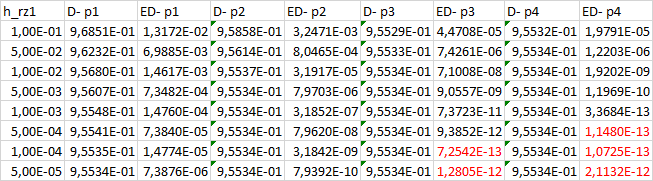
\includegraphics{Lab2/charts/rz1_log_Db_dane.png}

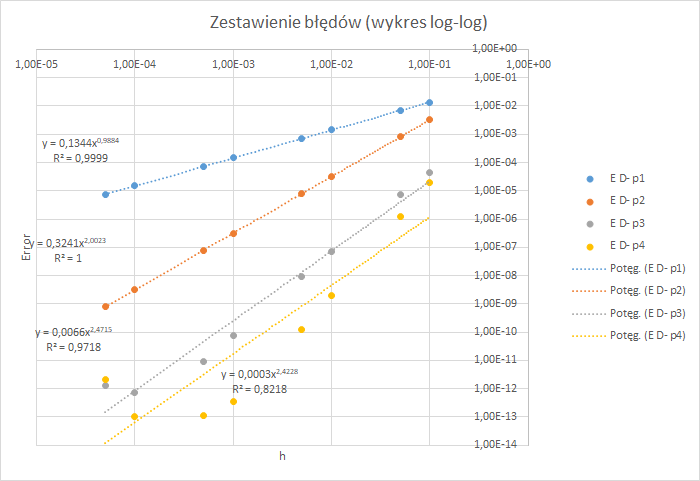
\includegraphics{Lab2/charts/rz1_log_Db.png} 
\newpage


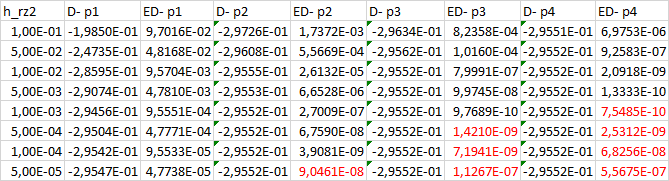
\includegraphics{Lab2/charts/rz2_log_Db_dane.png}

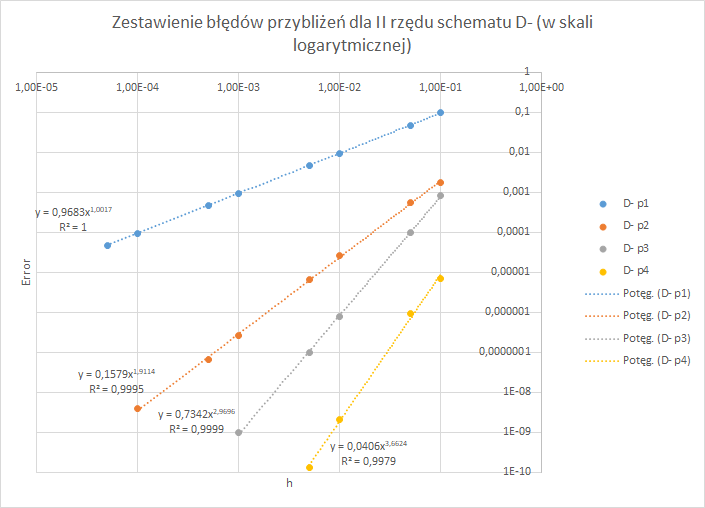
\includegraphics{Lab2/charts/rz2_log_Db.png}
\newpage


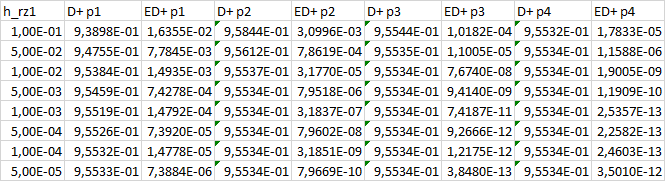
\includegraphics{Lab2/charts/rz1_log_Df_dane.png}

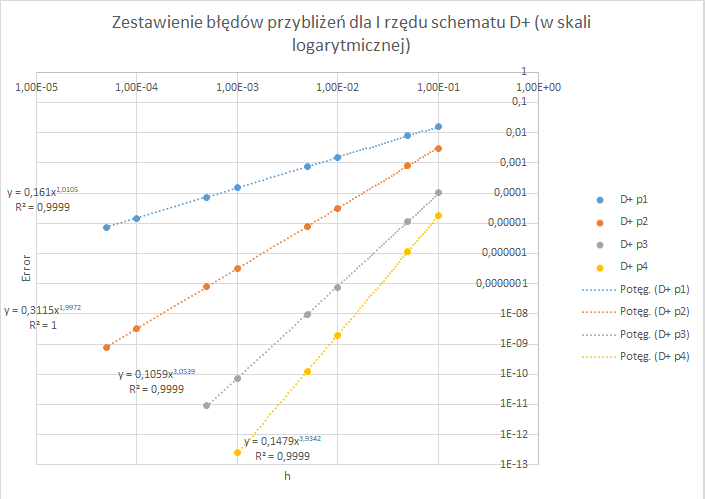
\includegraphics{Lab2/charts/rz1_log_Df.png}
\newpage


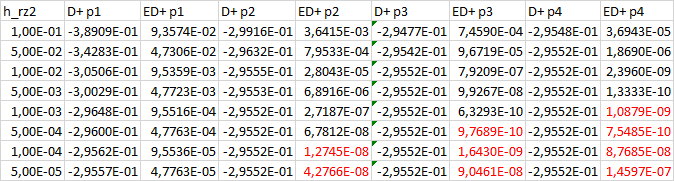
\includegraphics{Lab2/charts/rz2_log_Df_dane.png}

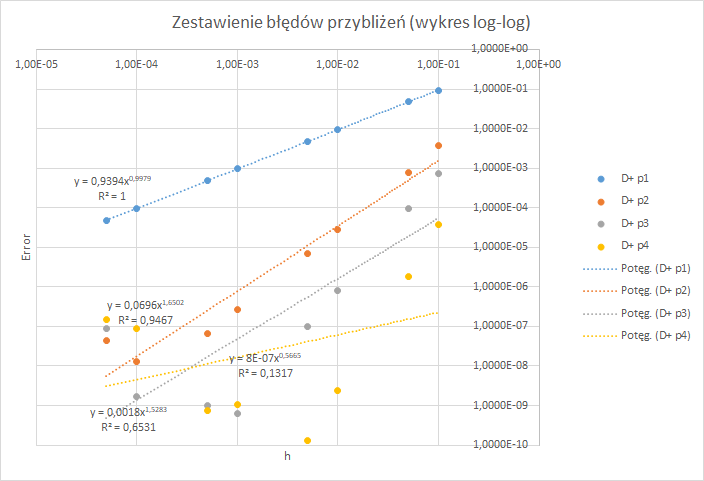
\includegraphics{Lab2/charts/rz2_log_Df.png}
\newpage


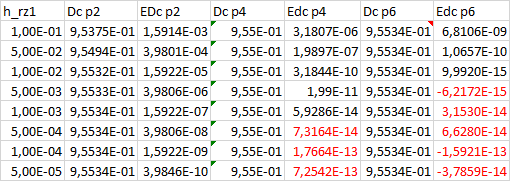
\includegraphics{Lab2/charts/rz1_log_Dc_dane.png}

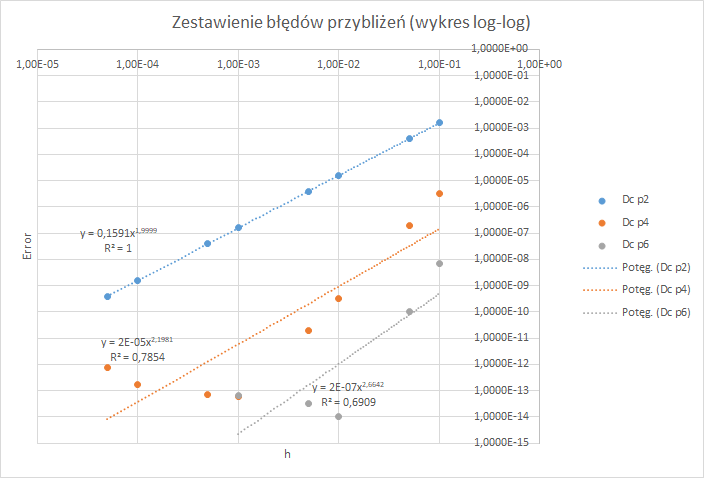
\includegraphics{Lab2/charts/rz1_log_Dc.png}
\newpage


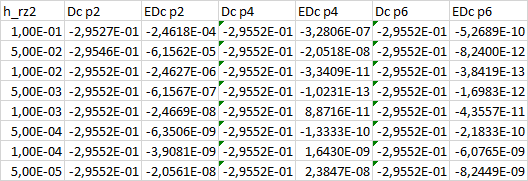
\includegraphics{Lab2/charts/rz2_log_Dc_dane.png}

Zestawienie błędów przybliżeń dla II rzędu schematu Dc na wykresie log-log nie jest możliwe. 

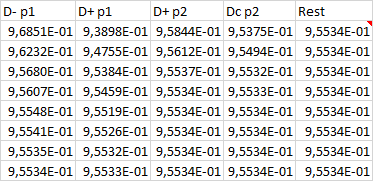
\includegraphics{Lab2/charts/rz1_log_e_dane.png}

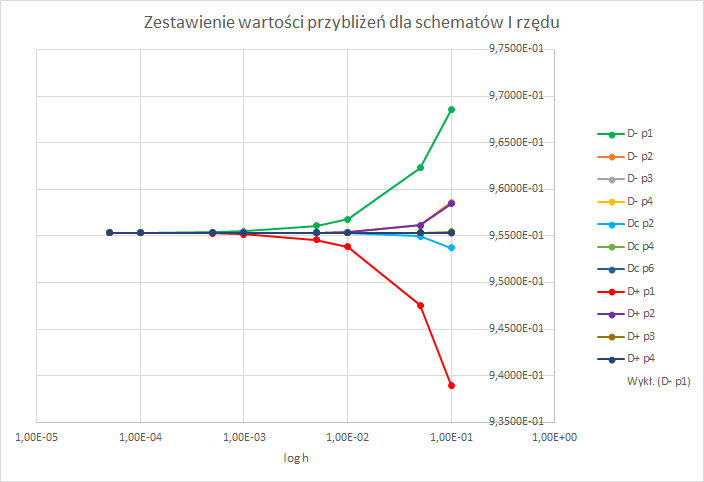
\includegraphics{Lab2/charts/rz1_log_e.png}
\newpage


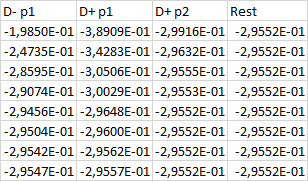
\includegraphics{Lab2/charts/rz2_log_e_dane.png}

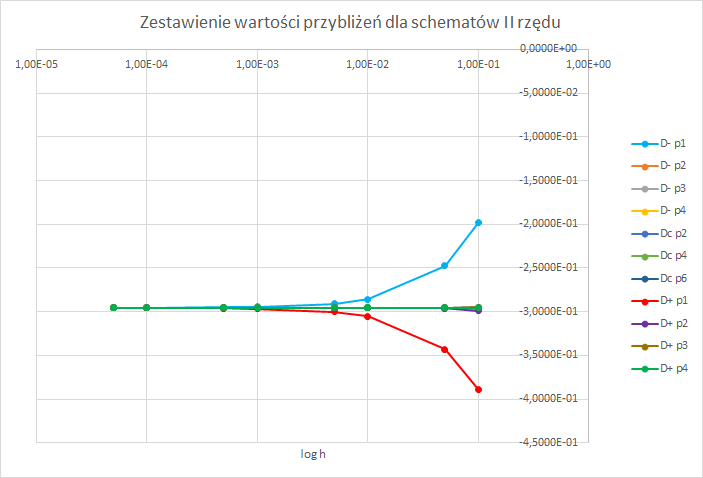
\includegraphics{Lab2/charts/rz2_log_e.png}
\newpage


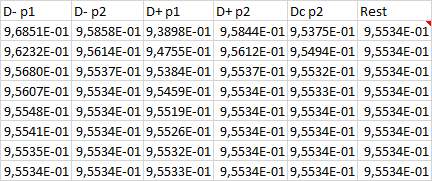
\includegraphics{Lab2/charts/rz1_e_dane.png}

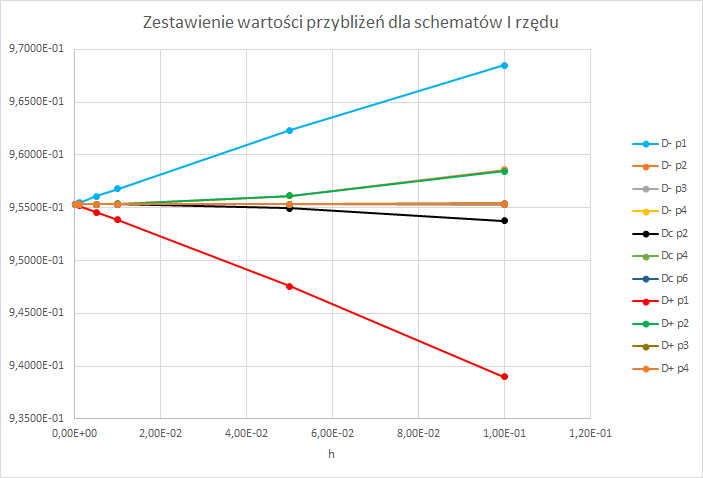
\includegraphics{Lab2/charts/rz1_e.png}
\newpage


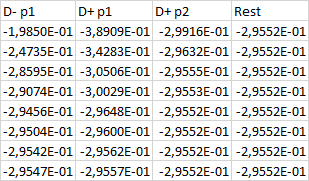
\includegraphics{Lab2/charts/rz2_e_dane.png}

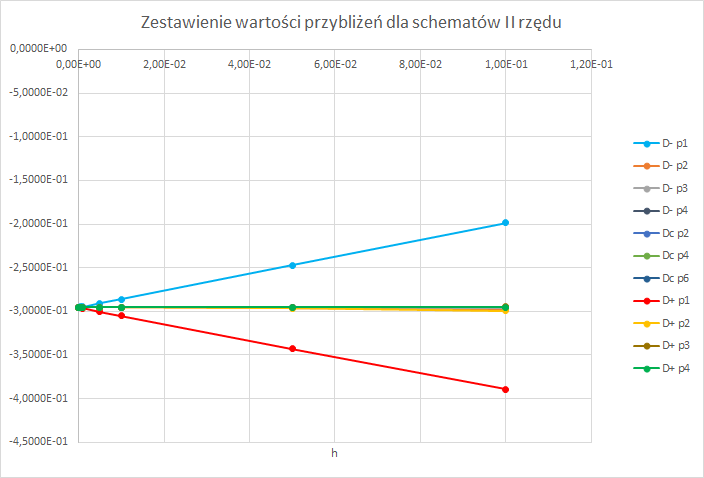
\includegraphics{Lab2/charts/rz2_e.png}



